\graphicspath{{figures/chapter-ocean-heat-carbon/}} % Specifies the directory where pictures are stored

\chapter{Ocean heat and carbon variability}
\label{cha:ocean_heat_carbon}

\begin{quotation}
  Most of the work contained in this chapter is based upon \textit{Thomas et al, 2017},
  submitted to in \emph{Journal of Climate}.
\end{quotation}

\section{Introduction}
The global ocean is an important component of the climate system. Holding far more
heat and carbon than the atmosphere, it is an
important sink for anthropogenic carbon and heat generated from greenhouse gas
emissions. Observational estimates suggest that as of 1995, the ocean has been
responsible for the uptake of approximately 100 Pg of anthropogenic carbon
\citep{Khatiwala2012,Sabine2004,Waugh2006}. Temperature observations have also
been used to estimate that the upper 2000 m of the ocean has been a sink for
15$\times$10$^{\mathrm{22}}$ J of excess heat \citep{Levitus2009} between the
years 1975--2005. Additionally, \citet{Frolicher2015} demonstrated that in
climate model simulations the Southern Ocean is an important region for oceanic
uptake of anthropogenic carbon and heat. They estimate that 30\% of
anthropogenic carbon and 75\% of anthropogenic heat that enters the ocean does
so south of 30$^{\circ}$S.

However, changes in the circulation due to both anthropogenic forcing and
natural variability may play an important role in heat and carbon uptake. Many
studies have examined how changes in Southern Ocean circulation impact ocean
carbon content \citep{Sarmiento1984,Sarmiento1996,Marinov2008}. Between the
1980's to early 2000's, multiple studies linked an acceleration of the
wind-driven Southern Ocean overturning with the resulting increase in upwelling
of carbon-rich waters resulting in a decrease in the Southern Ocean
CO$_{\mathrm{2}}$ sink despite an increase in atmospheric CO$_2$
\citep{LeQuere2000h,Lovenduski2007,Lenton2009}. More recently however,
observational studies have suggested this weakening of the Southern Ocean carbon
sink has reversed~\citep{Landsch2015,Devries2017}, highlighting the importance
of understanding natural variability.
Finally, in many models, Weddell Sea deep convection has been
determined to cause large fluctuations in ocean heat \citep{Latif2013,
DeLavergne2014a} and carbon content \citep{Bernardello2014}. While significant
effort has gone into understanding the net uptake of both heat and carbon, less
research has focused on the natural fluctuations of heat and carbon content
associated with longer (decadal-to-centennial) timescales of variability.

It is additionally important to examine heat and carbon variations together. A
recent paper by \citet{Winton2013} showed that the impacts on heat and carbon
uptake are different in response to changing ocean circulation. A change in
ocean circulation has a larger influence on oceanic heat uptake than carbon
uptake. This supports the results of \citet{Banks2006} and \citet{Xie2012} who
show that temperature in the ocean does not in fact behave as a passive tracer.

While studies have focused on the forced response of oceanic heat and carbon and
have demonstrated that heat and carbon have different storage and uptake
patterns, we are unaware of any studies that have explored the un-forced
co-variability of heat and carbon content. In this paper, we investigate natural
variability of both heat and carbon content in multiple simulations of an
Earth-system model. We examine the magnitude and frequency of the variability in
global heat and carbon content in simulations with various
mesoscale mixing parameter settings. We then look more closely at the regional
and spatial patterns of variability and finally, we propose possible mechanisms
that drive this variability. Varying the mesoscale mixing parameters allows us
to test the sensitivity of the patterns of variability and the mechanisms
driving this variability. This analysis aims to help understand the magnitude
of natural variability and provide a context with which to view anthropogenic
trends. Additionally it aids in the understanding of how carbon and heat vary
with respect to each other.


Descriptions of the model used and quantities examined is found in section
~\ref{section:methods}. Section~\ref{section:Temporal and Spatial Variations in
Heat and Carbon Content} discusses the temporal and spatial variability in heat
and carbon content. The mechanisms driving this variability are examined in
section~\ref{section:Mechanisms}, and conclusions are in section
~\ref{section:conclusions}.





% METHODS


\section{Methods}
\label{section:methods}
\subsection{Model and Simulation Descriptions}
We use the GFDL ESM2Mc \citep{Galbraith2011}, a coarse resolution configuration
of the GFDL ESM2M \citep{Dunne2012}. The model has an atmospheric resolution of
3.875$^{\circ} \times$ 3$^{\circ}$ with 24 vertical levels. The ocean model is
non-Boussinesq, using pressure as the vertical coordinate, and has a resolution
of 3$^{\circ} \times$ 1.5$^{\circ}$ and 28 vertical levels. Despite its
relatively coarse resolution, ESM2Mc has a realistic simulation of the Southern
Annular Mode \citep{Galbraith2011}, response of Southern Hemisphere winds to an
ozone hole \citep{Seviour2017}, and El Ni\~{n}o Southern Oscillation
\citep{Russell2014}. The vertical tracer diffusion coefficient ($K_v$) value is
set within the KPP module. The value increases with depth and buoyancy forcing.
When the water column is statically unstable the value can exceed 4 m s$^{-2}$
which implies an equilibration time of approximately 5 days even for a water
column that is 4000 m deep. The oceanic model also has a coupled
biogeochemical module referred to as the Biogeochemistry with Light Iron
Nutrients and Gases (BLING) model \citep{Galbraith2010}. Although this module
uses a highly parameterized biological cycle, it predicts patterns of carbon and
oxygen change in response to global warming that are very similar to a more complex
biogeochemistry simulation in ESM2M \citep{Small2014}.

Because of the coarse resolution, processes associated with oceanic eddies are
parameterized. The mesoscale advection of tracers along isopycnals is
parameterized using the Gent-McWilliams parameterization scheme \citep{Gent2010}.
The diffusion coefficient, A$_{\mathrm{GM}}$, varies spatially depending on the
meridional gradient of the vertical shear between 100 m -- 2000 m. A default
minimum and maximum value of A$_{\mathrm{GM}}$ is imposed at 200 m$^2$s$^{-1}$
and 1400 m$^2$s$^{-1}$ respectively. Additionally, the along-isopycnal diffusion
(neutral diffusion) by mesoscale eddies is parameterized using a coordinate
rotation method \citep{Redi1982a}. The neutral diffusion coefficient,
A$_{\mathrm{redi}}$, is set to a spatially constant value of 800 m$^2$s$^{-1}$
by default.

The model was initialized using the World Ocean Atlas present-day observations of
temperature, salinity, and nutrients and was run for 1500 years with
pre-industrial (1860) values of greenhouse gases and aerosols. An additional 500
years were simulated using the default value of A$_{\mathrm{redi}}$
(800 m$^2$s$^{-1}$) and this simulation is referenced as the \textit{control}
simulation. At year 1500, the model was branched to produce two more
500-year simulations using different, constant values of
A$_{\mathrm{redi}}$ = 400 and 2400 m$^2$s$^{-1}$.
These runs are referred to as the \textit{low eddy diffusion} and
\textit{high eddy diffusion} runs respectively. As discussed in
\citet{Pradal2014} and \citet{AnandGnanadesikan2015}, the value of
A$_{\mathrm{redi}}$ varies significantly across modern climate models, which
tend to use values lower than observational estimates \citep{Ollitrault2002}.
The range of values used here is comparable to those seen in the CMIP5 model
suite. One final 500-year simulation was conducted by branching the control run
and changing the minimum value of the mesoscale eddy advection coefficient,
A$_{\mathrm{GM}}$, to be 600 m$^2$s$^{-1}$ while maintaining the default value
of A$_{\mathrm{redi}}$ (800 m$^2$s$^{-1}$). This is referred to at the
\textit{high eddy advection} simulation.

Figure~\ref{fig:climatology} shows the winter-time climatologies (JJA) for various
Southern Hemisphere metrics with comparison to observations for all simulations.
The Southern Ocean temperature (Figure~\ref{fig:climatology} (a)) in the surface
layer is biased warm for all simulations. Additionally, all simulations except
the \textit{high eddy diffusion} simulation have subsurface temperatures exceeding
the observations. Similarly, the modeled surface salinity
(Figure~\ref{fig:climatology} (b)) is biased fresh for all simulations except the
\textit{high eddy diffusion} simulation. Figure~\ref{fig:climatology} (c) shows the
profile of density stratification strength ($\sigma_0 - \sigma_0^{\mathrm{1500m}}$).
The model simulations envelop the observational density stratification with the
\textit{high eddy advection} simulation having the strongest density
stratification and the \textit{high eddy diffusion} simulation having the weakest
stratification. The comparison of the modeled Southern Hemisphere westerly
wind stress with the ERA-Interim westerly wind stress is shown in
Figure~\ref{fig:climatology} (d). All the model simulations underestimate the
strength of the wind stress south of 40$^{\circ}$S and have an equatorward-biased
peak in the wind stress. Finally comparison with the observational sea ice-extent
is shown in Figure~\ref{fig:climatology} (e). All simulations under estimate the
sea ice extent in all months except the \textit{high eddy advection} simulation
which has accurate sea ice extent values in the austral spring.

\begin{figure}
\centering
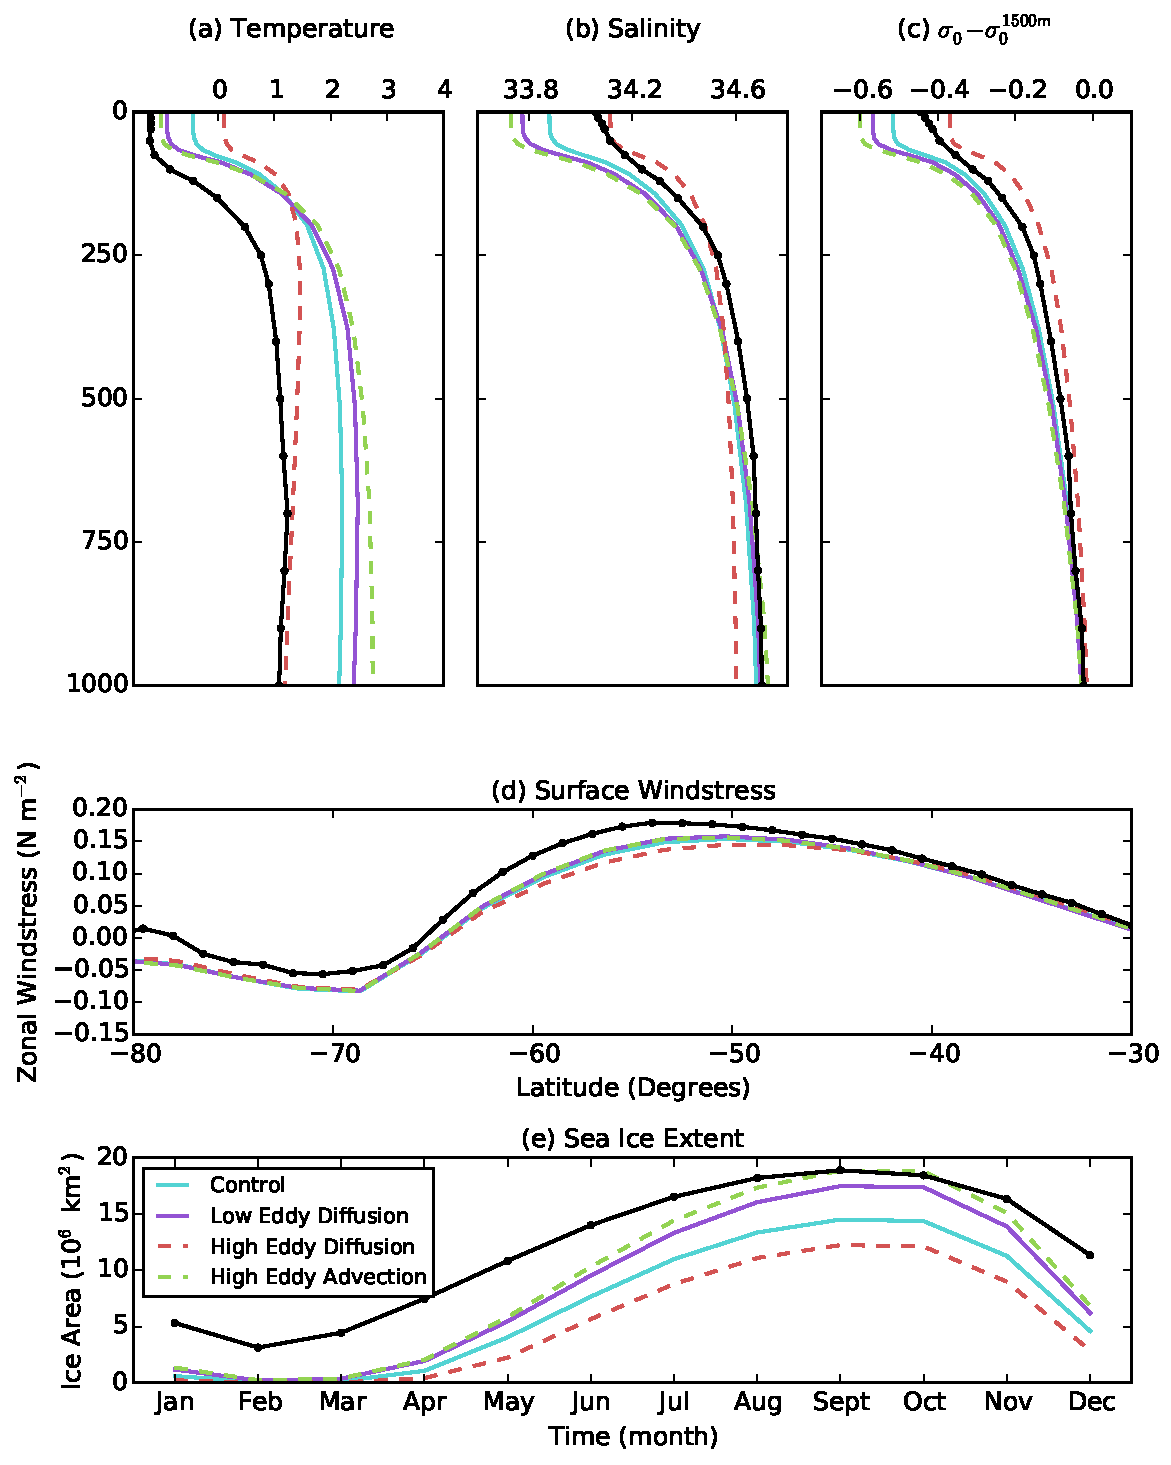
\includegraphics[width=33pc]{figure1.pdf}
\caption{Comparison of control (blue), low eddy diffusion (purple), high eddy
diffusion (red), and high eddy advection (green) simulations. JJA Southern Ocean
(60--90$^{\circ}$S) (a) temperature
(b) salinity and (c) density stratification
($\sigma_0 - \sigma_0^{\mathrm{1500m}}$). (d) JJA zonal surface wind stress
and (e) Antarctic sea ice extent. Observational data for each metric is shown in
black. Temperature, salinity, density stratification are estimates from the 2001
World Ocean Atlas 2001 dataset \citep{Boyer2002}. Surface wind stress are from ERA-Interim and averaged
between 1979--2015. Sea extent is calculated using the National Snow and Ice Data
Center Sea Ice Index \citep{Fetterer2016}}
\label{fig:climatology}
\end{figure}

The various $A_{\mathrm{redi}}$ simulations are discussed at length in
\citet{Pradal2014} and \citet{AnandGnanadesikan2015}, which examine the mean
climate response and sensitivity of anthropogenic carbon uptake to changing the
A$_{\mathrm{redi}}$ parameter. Here instead, we use the various simulations to
test the robustness of the mechanisms driving the co-variability of heat and
carbon. Because the different simulations have varying Weddell Sea  convective
variability (similar to the spread in CMIP5 models, see below), we can see if
convection alters the mechanisms driving the co-variability of heat and carbon
in this model. Unlike the CMIP5 suite where differences in biological models,
atmospheric radiation code, and sea ice formation contribute to intermodel
spread, our simulations differ only in the mesoscale parameterizations to
isolate the influence of Weddell Sea convection on the co-variability of heat
and carbon content.

\subsection{Heat and Carbon Content}
\label{subsection:Methods Heat and Carbon Content}
Heat and carbon content are calculated globally and regionally. The oceanic heat
content (H) is calculated using the subsurface potential temperature ($\theta$), and
integrated globally:

\begin{equation}
  H_{global} = \sum_{k = 0}^{bottom} \sum_{j = -90}^{90} \sum_{i=0}^{360} \rho
  c_p \theta \delta x_i \delta y_j \delta z_k
\end{equation}

Similarly, carbon content is calculated using Dissolved Inorganic Carbon (DIC)
concentration and integrated globally:

\begin{equation}
  C_{global} = \sum_{k = 0}^{bottom} \sum_{j = -90}^{90} \sum_{i=0}^{360} \rho
  [DIC] \delta x_i \delta y_j \delta z_k
\end{equation}

Because the oceanic heat and carbon reservoirs are so large ($150,000\times10^
{22}$ J and $37,000$ PgC, respectively), and the natural variability relatively
small ($\pm3\times10^{22}$ J and $\pm3$ PgC, respectively), we express the
variability as an anomaly from the climatological mean.

\subsection{Surface Heat Flux}
\label{subsection:Surface Heat Flux Analysis}

We determine the surface heat flux by vertically integrating the vertical
diffusion term over the entire water column and subtracting the geothermal heat
flux from the sea floor:
\begin{equation}
\begin{split}
\sum_{k = 0}^{bottom} {\bigg( \rho_k c_{p} {\bigg(\frac{\partial \theta}{\partial t}
\bigg)_{vdiff}}\bigg)_k}\delta z_k
 -… Q_{geo} = \\
Q_{SW} + Q_{LW} + Q_{latent} + Q_{sensible} = Q_{surface}
\end{split}
\end{equation}

The advantage to defining the surface heat flux with this method, as opposed to
the model-calculated surface heat flux, is that we can determine the heat
lost to overlying sea ice in addition to the atmosphere as well as track heat
sinks such as the melting of snow.

\begin{figure}
\centering
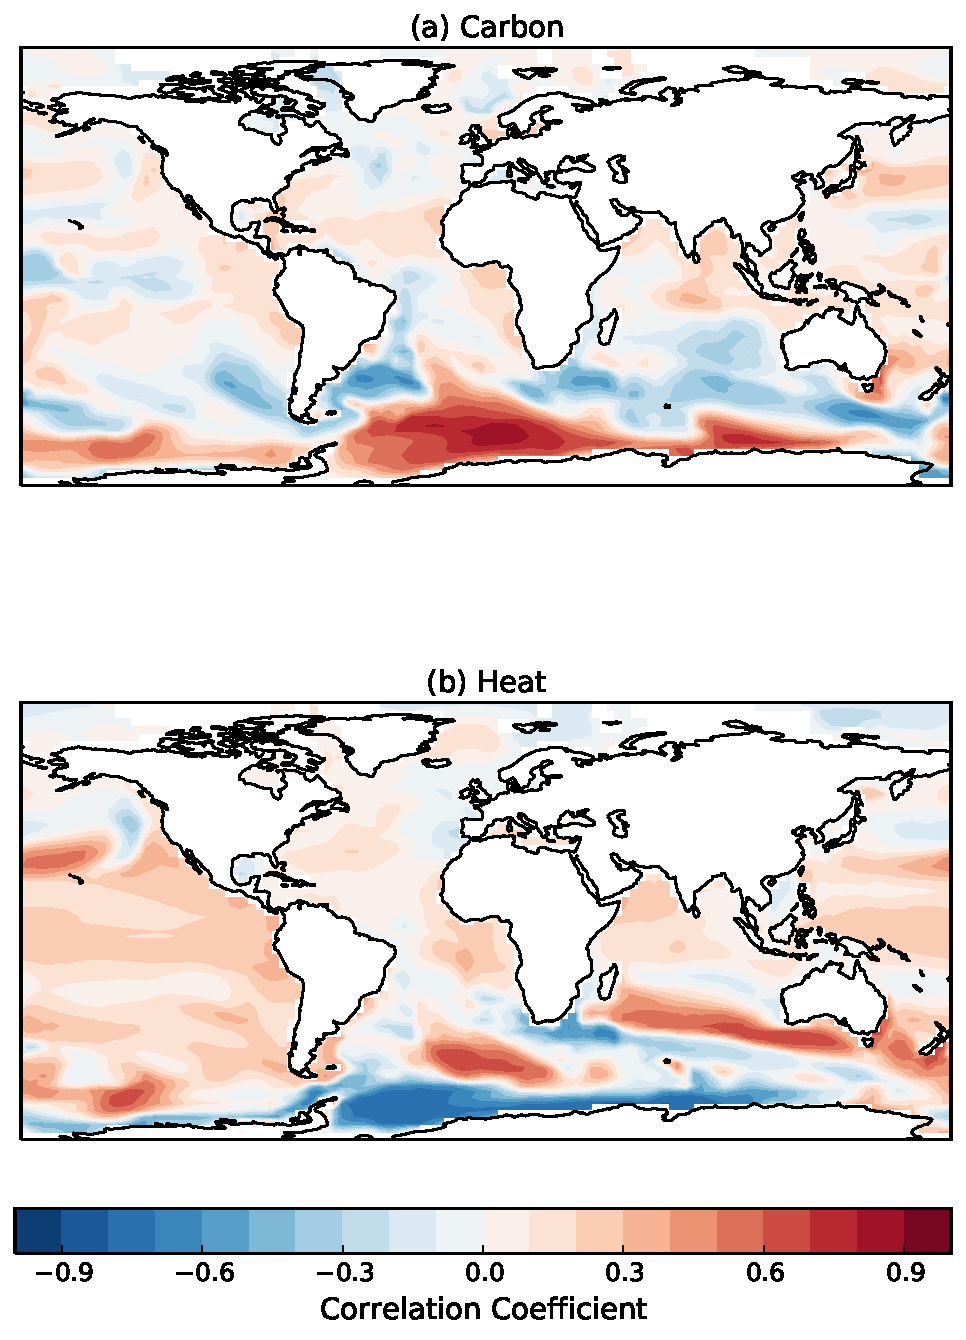
\includegraphics[width=19pc]{figure2.pdf}
\caption{Correlation between (a) vertically integrated carbon content at each
location and global carbon content and (b) vertically integrated heat content at
each location and global heat content for the control simulation
(A$_{\mathrm{redi}}$ = 800 m s$^{-2}$).}
\label{fig:heat_carbon_correlations}
\end{figure}

\subsection{Southern Ocean}
As has been previously documented \citep{DeLavergne2014a}, ESM2Mc has a
particularly active Southern Ocean. Deep convective events
occur often in the Southern Ocean, and have a sizable impact on the climate
system. \citet{Cabre} recently showed that Southern Ocean convective events in
this model have an impact on the Southern Hemisphere surface temperatures,
Hadley cell, and radiative balance. In light of the Southern Ocean influence in
this model, we first assessed the contribution of Southern Ocean variability to
global heat and carbon variability. Figure~\ref{fig:heat_carbon_correlations}
shows the correlation between vertically integrated carbon (heat) content at
each location with the global carbon (heat) content in the  \textit{control}
simulation. This initial analysis suggests the importance of  the Southern
Ocean, and particularly the Weddell Sea on global heat and carbon  variability
and will be more thoroughly examined in
section~\ref{section:Temporal and Spatial Variations in Heat and Carbon Content}.

%%%%%%%%%%%%%%%%%%%%%%%%%%%%%%%%%%%%%%%%%%%%%%%%%%%%%%%%%%%%%%%%%%%%%%%%%%%%%%%%
% RESULTS
%%%%%%%%%%%%%%%%%%%%%%%%%%%%%%%%%%%%%%%%%%%%%%%%%%%%%%%%%%%%%%%%%%%%%%%%%%%%%%%%
%% Section 1
\section{Temporal and Spatial Variations in Heat and Carbon Content}
\label{section:Temporal and Spatial Variations in Heat and Carbon Content}

%% Subsection 1

\subsection{Weddell Sea Convection}
In the mid-1970s, an anomalous opening in the sea ice in the Weddell Sea was
observed \citep{Carsey2009}. Named the Weddell Polynya, this large opening was
observed for three consecutive austral winters: 1974--1976. The polynya was
formed and maintained by vigorous convective mixing where the upward flux of
deep and relatively warm waters provided enough energy to melt the above sea
ice \citep{Gordon1982,Martinson1981}. This heat loss at the surface resulted in
subsurface cooling deep into the water column, depleting the subsurface heat
reservoir.

While a large feature like the Weddell Polynya has not been observed since and is considered to be a
rare event, these polynya events can be quite common in climate models. A recent
paper by \citet{DeLavergne2014a} quantifies these convective events in CMIP5
model preindustrial control simulations and shows the spread across models. They
find that some CMIP5 models have very little convection, while others have
constant deep convection, with most models lying somewhere in between.

Changing the mesoscale eddy parameterization in our model suite has a large
impact on the Weddell Sea deep convection. Figure~\ref{fig:convection} shows the
annually-averaged subsurface temperature as a function of time (colored
contours) and the annual mixed layer depth (black line) averaged over the
Weddell Sea (60--80$^{\circ{}}$S, 60$^{\circ{}}$W--0). The downward spikes in
mixed layer depth, and the concurrent decline in subsurface temperature indicate
the occurrence of a deep convective event. The simulations range from no
convection in the \textit{high eddy advection simulation} (Figure
~\ref{fig:convection} (d)), to constantly convecting in the \textit{high eddy
diffusion simulation} (Figure~\ref{fig:convection} (c)), with the
\textit{control} and \textit{low eddy diffusion} cases oscillating between
convective and non-convective periods (Figure~\ref{fig:convection} (a) and (b)).

When the neutral diffusion coefficient (A$_{\mathrm{redi}}$) is increased as in
the \textit{high eddy diffusion} simulation, the along isopycnal diffusive
mixing is increased. In the Southern Ocean where the isopycnals slope up to the
surface and the subsurface water is warmer than the surface ocean, this
increased along-isopycnal diffusion acts to decrease the vertical gradient in
temperature and salinity (also shown in Figure~\ref{fig:climatology} (a) - (c)).
This results in a lower subsurface temperature,
a weaker density contrast between deep and surface waters, less subsurface heat
build-up, and no large convective `events'
(Figure~\ref{fig:convection} (c)). Alternatively, a lower  neutral
diffusion coefficient as in the \textit{control} and \textit{low eddy diffusion}
simulations does the opposite: the along-isopycnal diffusive mixing is decreased
and subsurface heat is able to build up until a deep convective event occurs
(Figure~\ref{fig:convection} (a) and (b)).

Changing the eddy advection coefficient
(A$_{\mathrm{GM}}$) on the other hand impacts the slope of the isopycnal
surfaces. As shown in \citet{Gent2010d}, increasing A$_{\mathrm{GM}}$ acts to
flatten the isopycnal surfaces and reduce vertical exchange. In the Southern
Ocean where the isopycnals slope up to the surface, and the A$_{\mathrm{GM}}$
value is usually small, increasing the minimum value of A$_{\mathrm{GM}}$ thus
reinforces the vertical density gradient. The result is a build-up of subsurface
heat that continues to grow throughout the \textit{high eddy advection}
simulation. The reinforced density gradient is strong enough to suppress deep
convection throughout the 500-year simulation (Figure~\ref{fig:convection} (d)).

It is important to note that while the existence of subsurface heat build-up is
known to be important for the existence of deep convective events, it is not yet
known what mechanism initiates deep convection in the model or sets the
timescales for convective variability. We have found, however, that by changing
these parameterizations, we are able to span the range of convective variability
seen in CMIP5 models as shown in \citet{DeLavergne2014a} without the
additional complications introduced by different representations of atmospheric
processes and biological cycling. In this paper we will use these different
convective states of the model to identify the impact convective variability has
on both carbon and heat in the Southern Ocean and globally.


\begin{figure}
\centering
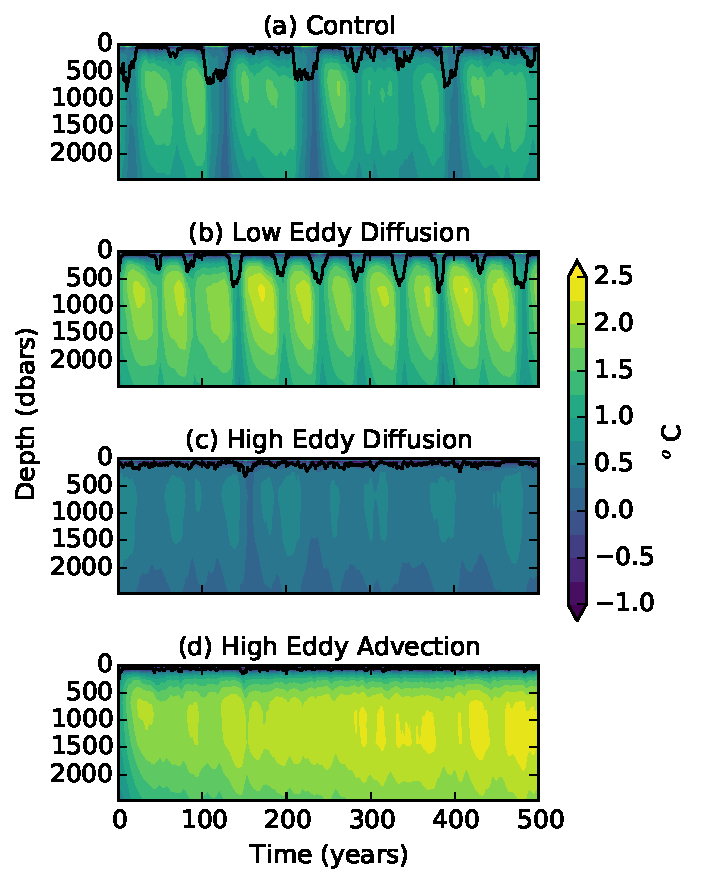
\includegraphics[width=19pc]{figure3.pdf}
\caption{Annually averaged subsurface temperature (color contours) and mixed
layer depth (solid black line) averaged over Weddell Sea for (a) Control
simulation (A$_{\mathrm{redi}}$ = 800 m s$^{-2}$), (b) Low Eddy Diffusion simulation
(A$_{\mathrm{redi}}$ = 400 m s$^{-2}$), (c) High Eddy Diffusion simulation
(A$_{\mathrm{redi}}$ = 2400 m s$^{-2}$), and (d) High Eddy Advection simulation
(GM$_{\min}$ = 600 m s$^{-2}$).}
\label{fig:convection}
\end{figure}

\subsection{Global Heat and Carbon Variability}
We first aim to understand the variability in global oceanic heat and carbon
content in the \textit{control} simulation. The time-series of global carbon and
heat content anomaly is shown in Figure~\ref{fig:heat_carbon_convection} (a) and
(b). Both quantities show strong multi-decadal-scale variability, undergoing
strong fluctuations roughly every 50 years. The magnitude of global
carbon variability is about $\pm$ 3 PgC which accounts for only approximately
3\% of the estimated anthropogenic uptake of carbon over the past few decades
\citep{Khatiwala2012,Sabine2004,Waugh2006}. The variability in global heat
content on the other hand is about $\pm$ 3 $\times 10^{22}$ J. This is a much
larger percentage (20\%) of the estimated uptake of anthropogenic in heat recent
decades \citep{Levitus2009}. Figure~\ref{fig:heat_carbon_convection}
(c) shows the time-series of Weddell Sea (WS)
subsurface temperature (averaged between 1500 m and 2500 m). This quantity has
been shown to be a good proxy for WS deep convection since the subsurface
temperature is significantly decreased during convective events \citep{Bernardello2014}.
Comparing the time-series of the WS subsurface temperature to those of
global heat and carbon anomalies, it is apparent that there is a strong
relationship. In the control simulation, the WS subsurface temperature explains
61\% and 35\% ($r^2$) of the variance in global heat content and carbon content
respectively (Table~\ref{t1}), with the strongest correlation occurring at time
lag = 0. The correlation between WS subsurface temperature and global heat and
carbon content is also high for the \textit{low eddy diffusion} simulation,
while the relationship is less strong (yet significant) for the \textit{high
eddy diffusion} and \textit{high eddy advection} simulations (Table~\ref{t1}).
These results suggest that WS convection is closely tied to the global heat and
carbon content.

\begin{figure}
\centering
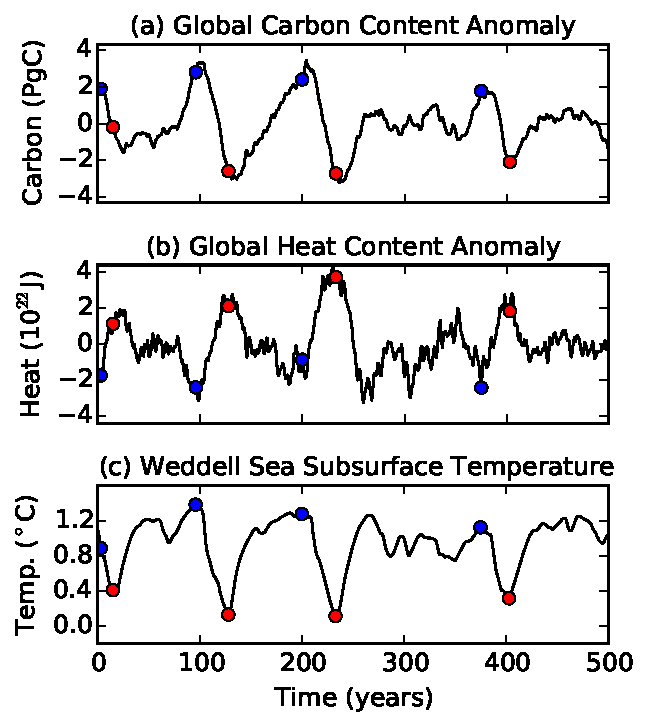
\includegraphics[width=19pc]{figure4.pdf}
\caption{Carbon content anomaly, heat content anomaly and Weddell Sea subsurface
temperature (averaged between 1500--2000 m, 0$^{\circ}$--60$^{\circ}$W,
60$^{\circ}$--80$^{\circ}$S) for control simulation. Blue circles indicate
beginning of convection and red circles indicate end of convection defined using
four strongest local maxima and minima in Weddell Sea Subsurface Temperature.}
\label{fig:heat_carbon_convection}
\end{figure}


\begin{table}[h]
\caption{Relationship between Weddell Sea subsurface temperature and global carbon
and heat content anomalies. All correlations are statistically significant from
0 (p = 0.005).}\label{t1}
\begin{center}
\begin{tabular}{lcc}
\hline
Simulation              & Carbon Content & Heat Content \\
\hline
 & \multicolumn{2}{c}{\textit{Correlations (r)}} \\
Control & 0.59 & -0.79   \\
Low Aredi & 0.61 & -0.56  \\
High Aredi & 0.49 & -0.20 \\
High GM$_{\mathrm{min}}$ min     & 0.12 & -0.24   \\
\end{tabular}
\end{center}
\end{table}

The global heat and carbon content anomaly time-series for all simulations is
shown in Figure~\ref{fig:heat_carbon_ts}. The
magnitude and frequency of heat and carbon content variability changes
substantially across the different simulations.  Comparing the time-series
of global carbon content and heat content anomalies in the control simulation we
find that they are anti-correlated ($r=-0.629$, Figure~\ref{fig:corr_coeff}).
Given that in this model, the global heat and carbon are primarily driven
by Southern Ocean variability and Southern Ocean convection acts to deplete the
Southern Ocean of both carbon and heat content, we would expect that global heat
and carbon content should vary together. Therefore it is surprising that the two
quantities are so strongly negatively correlated.

\begin{figure}
\centering
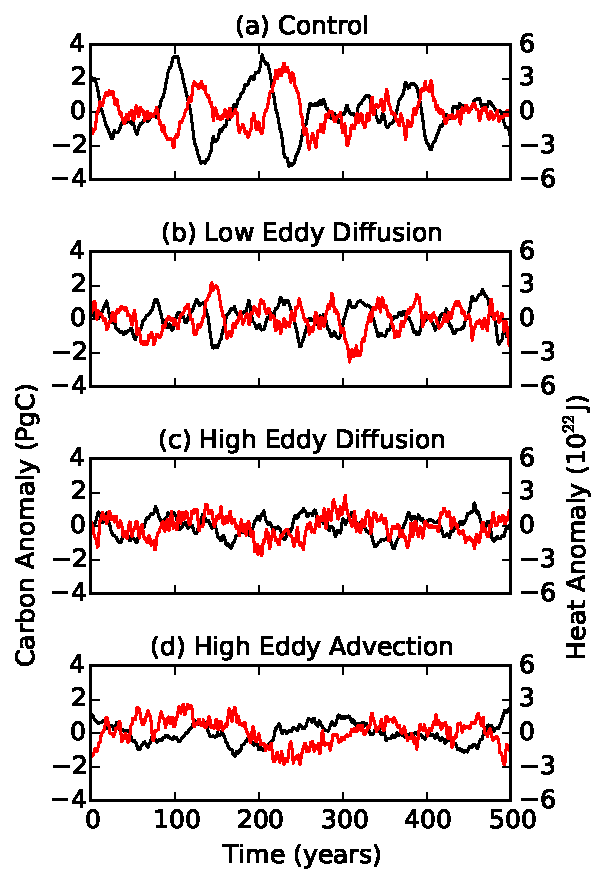
\includegraphics[width=19pc]{figure5.pdf}
\caption{Globally integrated carbon content anomaly (black) and heat content
anomaly (red) for (a) Control
simulation (A$_{\mathrm{redi}}$ = 800 m s$^{-2}$), (b) Low Eddy Diffusion simulation
(A$_{\mathrm{redi}}$ = 400 m s$^{-2}$), (c) High Eddy Diffusion simulation
(A$_{\mathrm{redi}}$ = 2400 m s$^{-2}$), and (d) High Eddy Advection simulation
(GM$_{\min}$ = 600 m s$^{-2}$).}
\label{fig:heat_carbon_ts}
\end{figure}

This anti-correlation relationship between global heat and carbon content is
consistent in the additional simulations as well (Figure~\ref{fig:heat_carbon_ts}).
Figure~\ref{fig:corr_coeff} shows the Pearson
correlation coefficient between global heat and carbon content for each
simulation. All of the simulations have a statistically significant negative
correlation between global heat and carbon exceeding -0.3. The two simulations
which oscillate between convective and non-convective periods (\textit{control} and \textit{low eddy
diffusion}) have stronger correlations at or exceeding -0.5. The fact that
significant anti-correlation is found for all simulations suggests that
the mechanisms causing this anti-correlation in global heat and carbon content
are not strongly dependent on the convective state in the WS.

\begin{figure}
\noindent
\centering
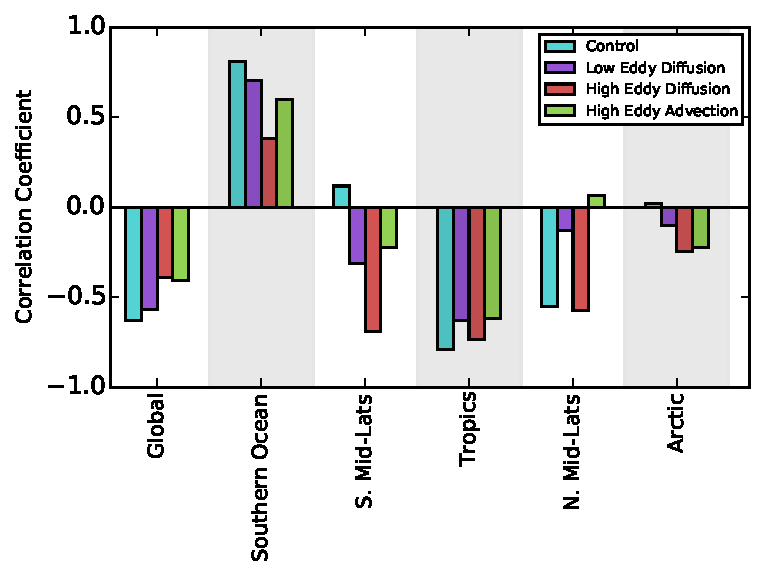
\includegraphics[width=33pc]{figure6.pdf}
\caption{Pearson correlation coefficients for integrated carbon content anomaly
versus integrated heat content anomaly for each region.}
\label{fig:corr_coeff}
\end{figure}

In light of these results, we find it helpful to divide these simulations up
into two classes: the \textit{low mixing simulations} which oscillate between
convective and non-convective periods (control and low eddy diffusion) and the
\textit{high mixing simulations} simulations which do not (high eddy diffusion
and high eddy advection). The low mixing simulations are characterized by a
build-up and subsequent release of abyssal heat content in the Southern Ocean
(Figure~\ref{fig:convection}). These two simulations also have very strong
oscillations in the global heat and carbon content, closely linked to the WS
convection. The high mixing simulations on the other hand do not show
this oscillation between subsurface build-up and release in the Southern Ocean,
but rather either constant depletion in subsurface temperature in the
\textit{high eddy diffusion} (Figure~\ref{fig:convection} (c)) or a constant
build-up of subsurface temperature in the \textit{high eddy advection}
(Figure~\ref{fig:convection} (d)). The lack of these oscillating convective
states results in smaller global heat and carbon variability
(Figure~\ref{fig:heat_carbon_ts}), and a weaker relationship (although
significant) between the WS and the global heat and carbon content.

To understand why the global heat and carbon are strongly anti-correlated, next
we look at the regional relationships between heat and carbon content.


%% Subsection 2
\subsection{Regional Heat and Carbon Variability}
To diagnose which regions significantly contribute to the observed variability
in global heat and carbon content, we break the global ocean into zonal bands:
the Southern Ocean (90$^o$S--55$^o$S), the southern mid-latitudes (55$^o$S--
20$^o$S), tropics (20$^o$S--20$^o$N), the northern mid-latitudes (20$^o$N--
60$^o$N), and the Arctic (60$^o$N--90$^o$N). These divisions were defined by the
zonal average of the zero wind-stress curl in order to isolate the dynamical
regions (not shown). The correlation coefficients
between heat and carbon content in each of these regions are also shown in
Figure~\ref{fig:corr_coeff}. The correlation coefficients give a sense of what
remains consistent across the simulations even with the different convective
states. The Southern Ocean has a strong positive correlation between heat and
carbon for all the simulations. Additionally, in the tropics there is a strong
negative correlation between heat and carbon for all the simulations. This
result suggests that the negative correlation in the tropics is key to
understanding the negative correlation between heat and carbon seen globally.

To get a better sense of which regions dominate the variability, we decompose
the global heat and carbon regionally by regressing the regional inventories of
heat and carbon against the global inventories of heat and carbon. We first
consider heat content in the \textit{control} simulation
(Figure~\ref{fig:linear_regression} (a), red dots). The regression highlights
the importance of three regions in contributing to the global heat content
signal: the Southern Ocean, southern mid-latitudes, and tropics. The Southern
Ocean regression coefficient has a magnitude similar to the southern
mid-latitudes and tropics, but the opposite sign. This indicates that the
variability in Southern Ocean heat content is being compensated by similar
magnitude variability in heat content in both the southern mid-latitudes and
tropics.

\begin{figure}
\noindent
\centering
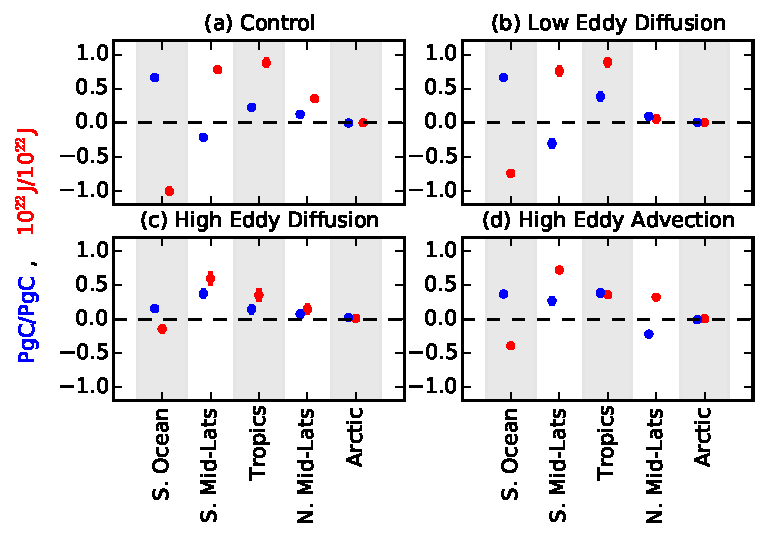
\includegraphics[width=33pc]{figure7.pdf}
\caption{Linear regression of each region's carbon content against global carbon
content (blue) and each regions heat content against global heat content (red).
Linear regression  95\% confidence interval is shown, but too small to be
discerned.}
\label{fig:linear_regression}
\end{figure}

The picture is nearly identical in the \textit{low eddy diffusion} simulation
(which also undergoes oscillations between convective and non-convective
states). The Southern Ocean heat content variability is compensated by similar
magnitude variability in both the southern mid-latitudes and tropics
(Figure~\ref{fig:linear_regression} (b)). However, the \textit{high mixing}
simulations are less clear. The regional heat content is dominated by the
southern mid-latitudes with weak compensation between the Southern Ocean
and tropics (Figure~\ref{fig:linear_regression} (c) and (d)).

The linear regression of regional carbon content
(Figure~\ref{fig:linear_regression}, blue dots), however, suggests that the
Southern Ocean carbon content variability contributes most towards the global
carbon content variability for all simulations. For the \textit{low mixing simulations},
there appears to be a compensation between the southern mid-latitude and tropical
carbon content variability. This compensation in regional variability is not seen
in the \textit{high mixing simulations} where the regression coefficients are both
positive for these two regions. Regardless of these differences, the Southern
Ocean is the region with the largest regression coefficient for all simulations.

The time-series of the regional variability for heat and carbon content compared
to the global heat and carbon content are shown in the supplemental information
as an additional way to visualize the offsetting variations in different regions.

This relationship between WS deep convection and Southern
Hemisphere surface warming is consistent with \citet{Bernardello2014} and
\citet{Cabre}. Both papers use the same GFDL model shown here in the control configuration to assess the
impact of convection on the climate system and both sets of analysis show
similar Southern Hemisphere surface warming in response to a convective event.
Specifically, \citet{Cabre} show that during these winter time convective events,
substantial warming occurs in the Southern Ocean, increasing sea surface
temperatures, decreasing sea ice and low clouds, and increasing solar radiation
absorption. The result is a substantial warming of the Southern Hemisphere surface
ocean and atmosphere. This atmospheric warming propagates to the rest of the
atmosphere almost instantaneously, changing the meridional temperature gradient
and altering the strength of the Hadley Cell in both hemispheres. For a more
detailed look at the teleconnections between the Southern Ocean convection and
tropical SST increases, we refer the reader to \citet{Cabre}.


\begin{figure}
\noindent
\centering
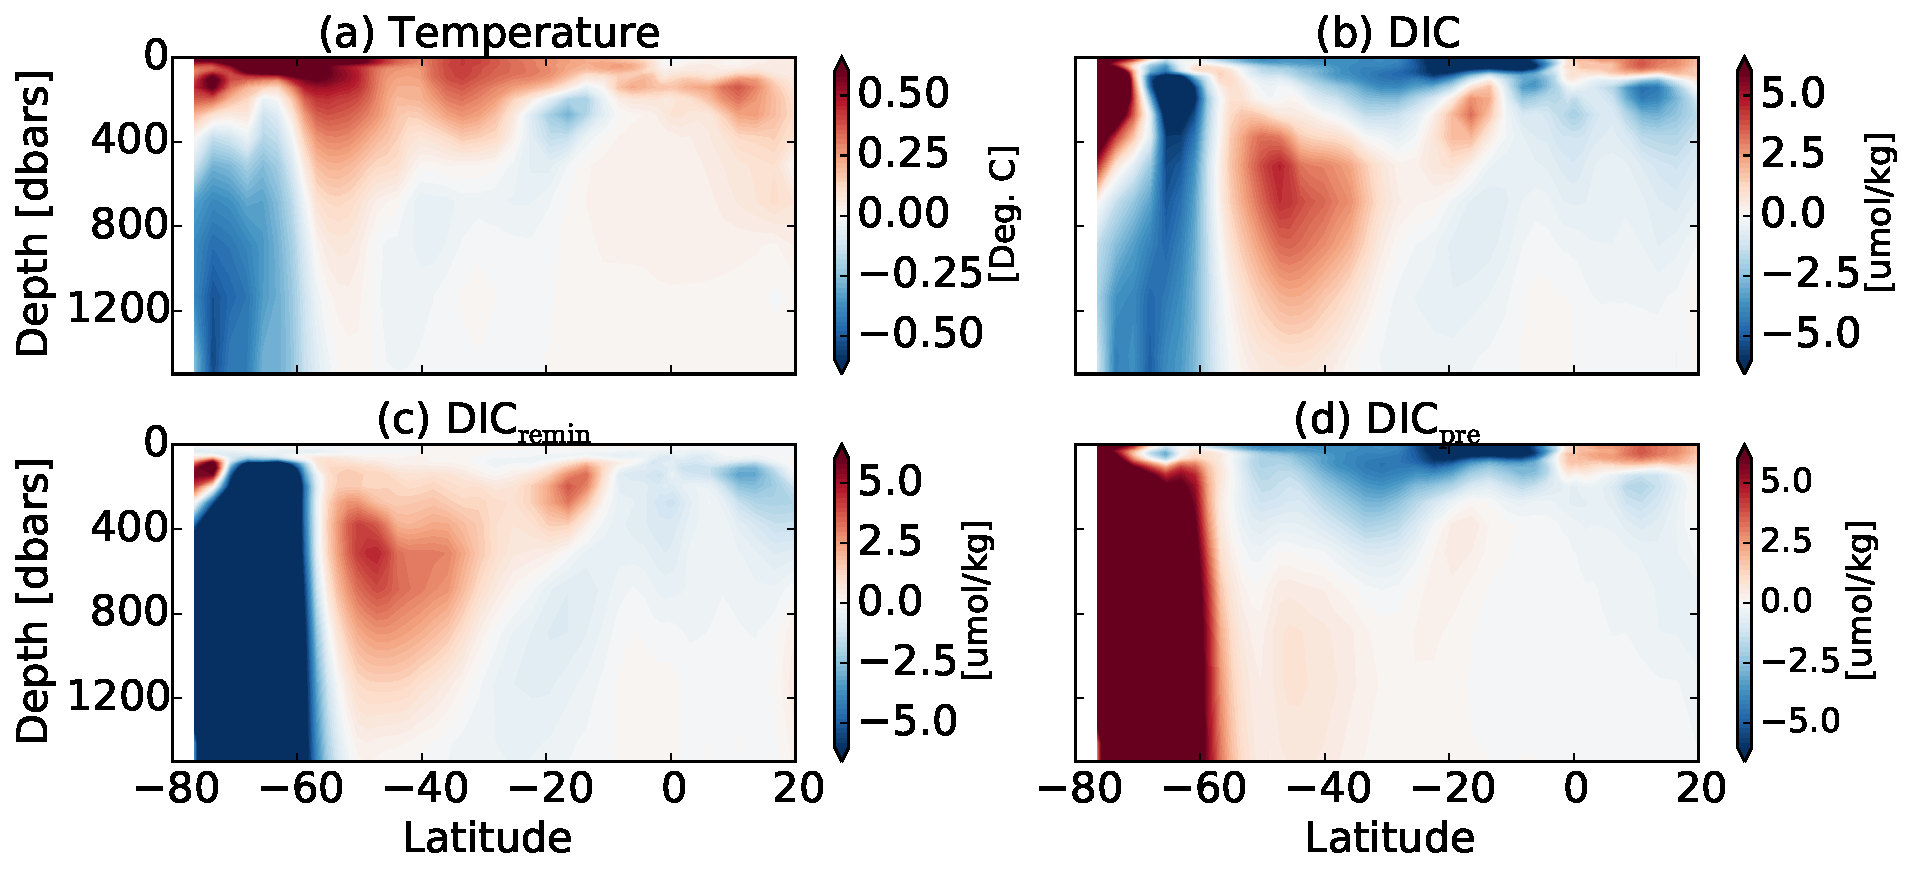
\includegraphics[width=33pc]{figure8.pdf}
\caption{Subsurface (a) potential temperature, (b) DIC, (c) remineralized DIC, and (d) preformed
DIC for convective year composite from control simulation. Only the surface ocean
is shown to highlight the strongest-magnitude features.}
\label{fig:subsurface}
\end{figure}



%%%%%%%%%%%%%%%%%%%%%%%%%%%%%%%%%%%%%%%%%%%%%%%%%%%%%%%%%%%%%%%%%%%%%%%%%%%%%%%%
% MECHANISMS
%%%%%%%%%%%%%%%%%%%%%%%%%%%%%%%%%%%%%%%%%%%%%%%%%%%%%%%%%%%%%%%%%%%%%%%%%%%%%%%%
\section{Mechanisms Driving Variability}
\label{section:Mechanisms}

In order to understand why global heat and carbon content are anti-correlated
we look more in depth at the mechanisms driving the regional variability of
these quantities.

\subsection{Heat Content Variability}
We first examine the variability of heat content. As shown for the \textit{control}
simulation subsurface temperature in Figure~\ref{fig:subsurface} (a), convection
acts to deplete the Southern Ocean of subsurface heat, and increase the surface
heat content in the southern mid-latitudes and tropics. These processes are more
explicitly shown in Figure~\ref{fig:heat_flux_fig}. Periods of convection
(highlighted in grey) are consistent with deepening of the mixed layer
(black line), a depletion of subsurface Southern Ocean temperature (green line),
an increase in Southern Ocean heat flux into the atmosphere (negative out of
ocean -- red line), and an increase in southern mid-latitude and tropical SST
(blue line). These processes are consistent in the \textit{low eddy diffusion}
simulation which  also oscillates between convective and non-convective periods
(not shown).

This relationship between WS deep convection and Southern
Hemisphere surface warming is consistent with \citet{Bernardello2014} and
\citet{Cabre}. Both papers use the same GFDL model shown here to assess the
impact of convection on the climate system and both sets of analysis show
similar Southern Hemisphere surface warming in response to a convective event.
Specifically, \citet{Cabre} show that during these winter time convective events,
substantial warming occurs in the Southern Ocean, increasing sea surface
temperatures, decreasing sea ice and low clouds, and increasing solar radiation
absorption. The result is a substantial warming of the Southern Hemisphere surface
ocean and atmosphere. This atmospheric warming propagates to the rest of the
atmosphere almost instantaneously, changing the meridional temperature gradient
and altering the strength of the Hadley Cell in both hemispheres. For a more
detailed look at the teleconnections between the Southern Ocean convection and
tropical SST increases, we refer the reader to \citet{Cabre}.

In this paper we show that the impact of this surface warming in the southern
mid-latitudes and tropics is strong enough to counteract the depletion of
subsurface heat in the Southern Ocean, resulting in a global increase in heat
content after WS convection.

\begin{figure}
\noindent
\centering
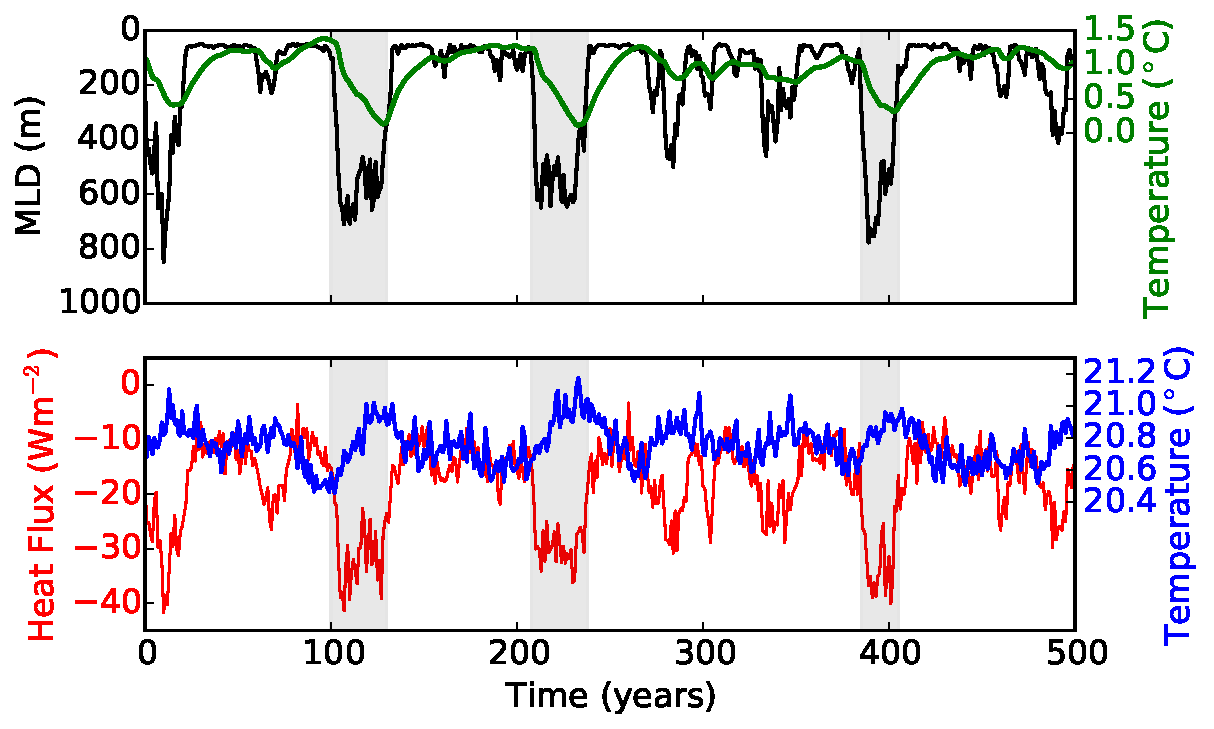
\includegraphics[width=33pc]{figure9.pdf}
\caption{Top: Weddell Sea subsurface temperature as in Figure
~\ref{fig:heat_carbon_convection} (green) and Weddell Sea mixed layer depth
(black). Bottom: Southern Ocean surface heat flux where positive indicates into
the ocean (red), Southern Hemisphere SST averaged between
0$^{\circ}$--55$^{\circ}$S (blue) for the control simulation.}
\label{fig:heat_flux_fig}
\end{figure}

\subsection{Carbon Content Variability}
Next we examine the regional mechanisms driving variability in carbon content in
order to understand the anti-correlation between global heat and carbon content.
Examining the \textit{control} simulation (Figure~\ref{fig:subsurface} (b)), we
see that during convection there is a strong subsurface depletion of DIC in the
Southern Ocean, an increase in subsurface DIC in the southern mid-latitudes, and
a further depletion of surface-layer DIC in the southern mid-latitudes to equator.
To understand these spatial patterns, we
break the DIC up into two components:
\begin{equation}
DIC = DIC_{pre} + DIC_{remin}
\end{equation}

where the preformed component (DIC$_{pre}$) is the DIC concentration of the
water at the ocean surface and the remineralized component (DIC$_{remin}$) is
the carbon concentration due to biological accumulation. DIC$_{pre}$ is set
equal to DIC in the mixed layer and is advected and mixed into the ocean
interior with biological sources and sinks set to zero. Thus by definition,
 DIC$_{remin}$ is zero within the mixed layer and represents the component of
 DIC in the interior that is due to biological sources and sinks.

When breaking the DIC down into its two components, we see that in
the Southern Ocean there is a very strong depletion of subsurface remineralized
carbon and a strong increase in preformed carbon (Figure~\ref{fig:subsurface}
(c) and (d)). This signal is consistent with deep convective mixing. The
increase in subsurface DIC$_{pre}$ occurs from mixing relatively high surface
DIC$_{pre}$ down into the subsurface and the decrease in DIC$_{remin}$ occurs from
mixing relatively high DIC$_{remin}$ from the subsurface to the surface layer.
Mixing these high DIC waters from the abyssal Southern Ocean to the surface
results in outgassing of CO$_2$ to the atmosphere (not shown) and the net result
is a reduction in subsurface DIC.

The depletion in surface DIC in the Southern Hemisphere tropical region on the
other hand is entirely due to a depletion in preformed DIC. This region also
experiences a strong warming thus reducing the solubility of CO$_{\mathrm{2}}$
within the surface waters and
limiting the amount of DIC that can be held by the water in equilibrium with the
atmosphere and at constant alkalinity. To verify that the reduction
in solubility is driving the subsequent decrease in DIC, we show the
DIC content versus heat content for the tropical region in
Figure~\ref{fig:heat_dicpre_scatter} (a). The strong negative relationship
supports the hypothesis that the variability in preformed DIC in this region is
driven by changes in solubility. Figure~\ref{fig:heat_dicpre_scatter} (a)
additionally shows the theoretical change in carbon content given a change in
heat content due to solubility alone (constant pCO$_{\mathrm{2}}$ and alkalinity
-- black line) with a slope of  -0.27 PgC/$10^{22}$J. This relationship is calculated using the relationship derived
in \citet{Gruber1996} and scaled to relate carbon content with heat content.
There is good agreement between this theoretical model and the linear regression of carbon content
versus heat content for this region, represented by the dashed grey line (linear slope
values, $m$, also shown on Figure~\ref{fig:heat_dicpre_scatter}),
 further supporting the hypothesis that carbon variability is consistent
with variability in solubility.

\begin{figure}
\noindent
\centering
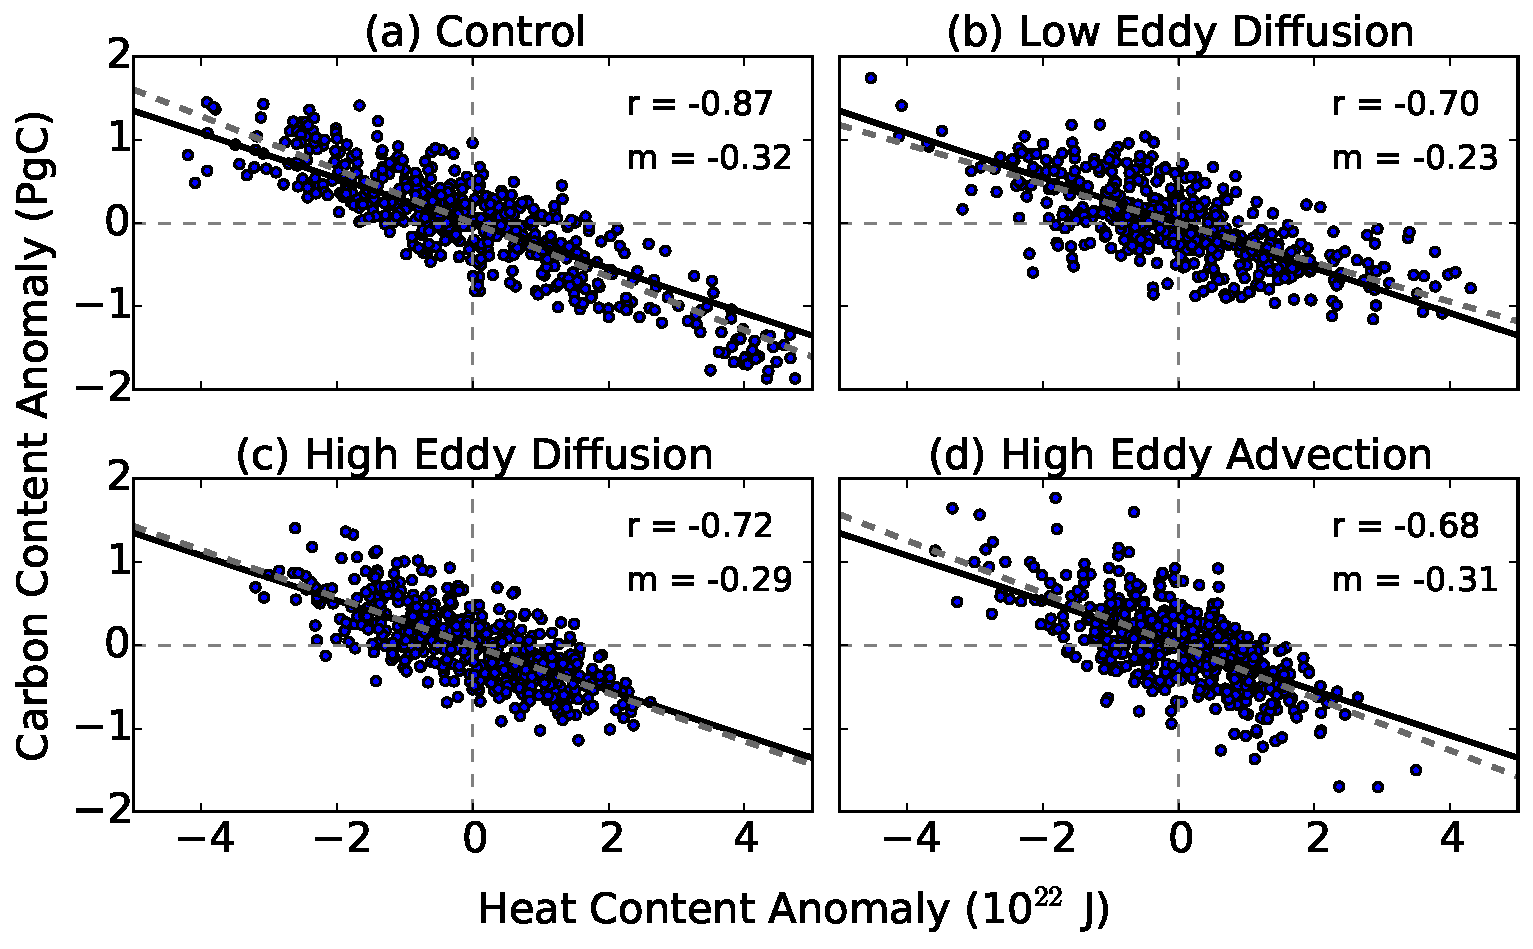
\includegraphics[width=33pc]{figure10.pdf}
\caption{Scatter of heat content anomaly vs preformed DIC integrated over the
tropical region for each simulation. Dashed grey linear line represents the linear fit of the carbon vs heat data with
slope, $m$, and pearson correlation coefficient $r$.
Solid black linear line represents the projected change
in carbon content given a change in heat content with constant alkalinity and
pCO$_2$ in equilibrium with the preindustrial atmosphere (scaled from \citet{Gruber1996}).
}
\label{fig:heat_dicpre_scatter}
\end{figure}

The above solubility mechanism appears to hold in all simulations
(Figure~\ref{fig:heat_dicpre_scatter} (b) -- (d)). All simulations have the same
negative relationship between preformed carbon content and heat content
integrated over the tropical region (20$^\circ{}$S -- 20$^\circ{}$N) with good
agreement with the scaled solubility line (black line). This result
suggests that the variability in DIC in this region is driven by variability
in the temperature-driven solubility, regardless of the high-latitude convective
variability.

Finally we examine the southern mid-latitude subsurface increase in DIC seen in
Figure~\ref{fig:subsurface} (b). Looking at the components of DIC, it is apparent that this
increase is entirely due to remineralized DIC. To understand why this increase
of remineralized DIC occurs, we correlate the remineralized DIC anomaly with ideal age
in the southern mid-latitude subsurface region (averaged between 40$^\circ{}$--
50$^\circ{}$S and 200--1000 m, Figure~\ref{fig:dic_remin_vs_age}). The ideal age
is a tracer in the model simulation which quantifies the mean time since the
water last had contact with the surface. The tracer is set to zero in the mixed
layer and ages at a rate of 1 yr yr$^{-1}$ after it leaves the mixed layer.
In all simulations, the remineralized DIC anomaly in this region is strongly correlated
with ideal age with Pearson
correlation coefficients exceeding 0.8 (Figure~\ref{fig:dic_remin_vs_age}).
Calculating the linear regression coefficient ($m$) between the remineralized
DIC and ideal age yields a rate of accumulation of remineralized DIC of
approximately 0.25 $\mu$mol kg$^{-1}$ yr$^{-1}$ for all simulations
(Figure~\ref{fig:dic_remin_vs_age}).
Comparing this rate of accumulation of remineralized DIC to the modeled local
remineralization rate ($jPO_4 \times$ 108 = 1.6 $\mu$mol kg$^{-1}$ yr$^{-1}$) we find that
the rate of accumulation of remineralized DIC in this region is significantly
less than the remineralization rate. The DIC found at a given point has
accumulated along many trajectories, some largely passing through surface waters
where the local remineralization rate is large, and some passing through deep
waters where the local remineralization rate is small. The low slope of the
relationship between DIC$_{remin}$ and age suggests that it is changes in the
fraction of waters taking deeper trajectories that is most important in
explaining the changes in Figure~\ref{fig:dic_remin_vs_age}.

\begin{figure}
\noindent
\centering
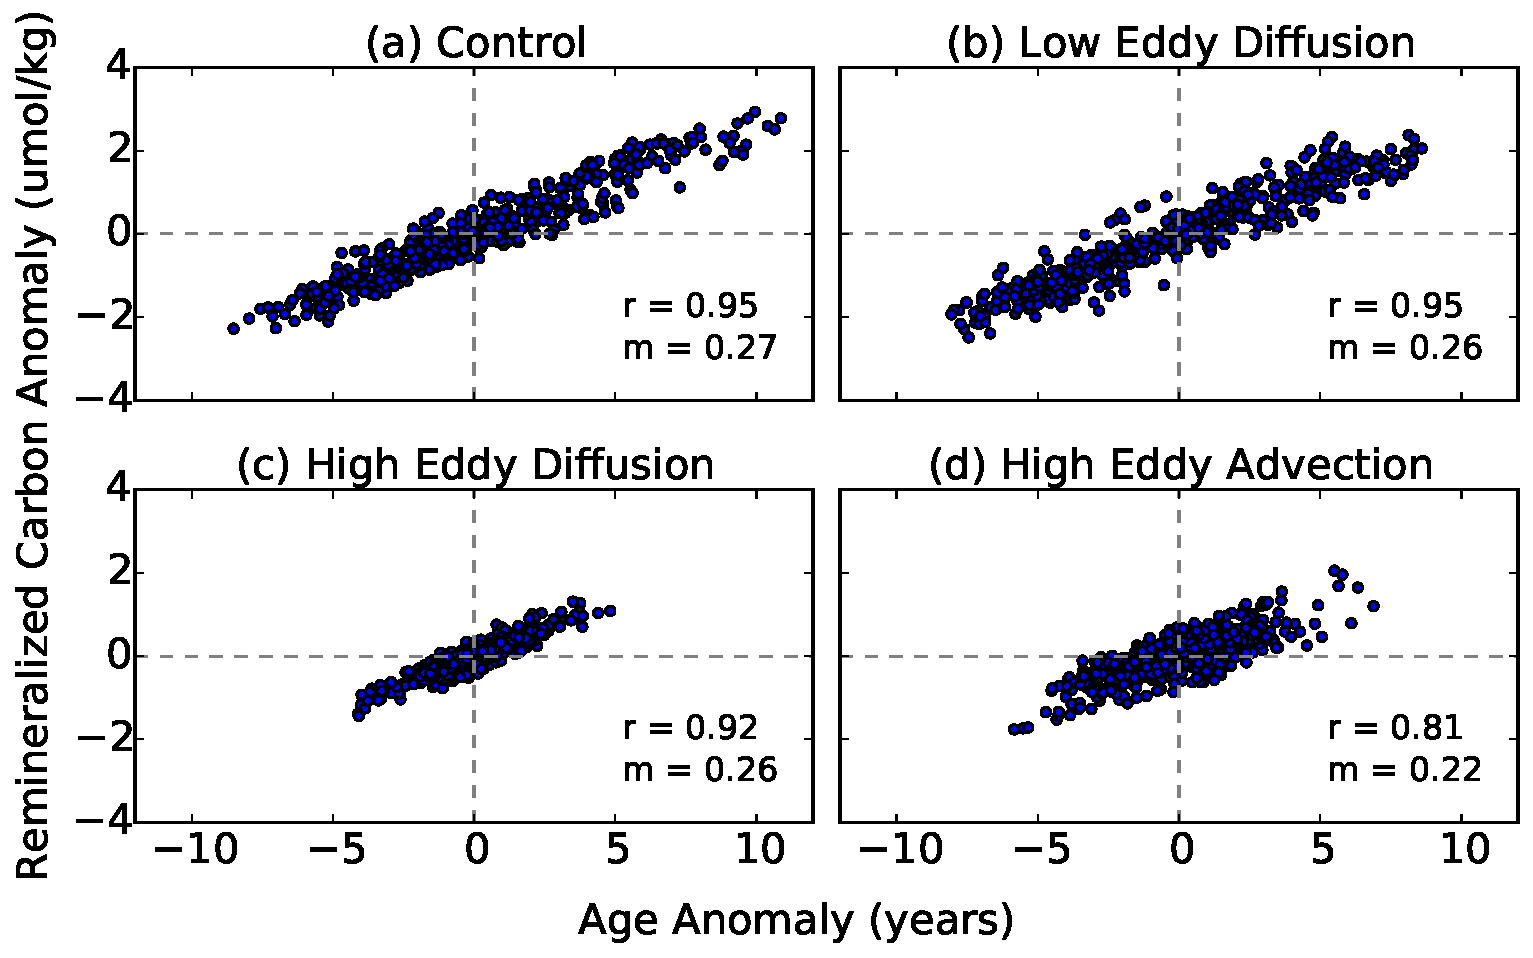
\includegraphics[width=33pc]{figure11.pdf}
\caption{Ideal age versus remineralized DIC for all simulations. Quantities are
averaged over latitudes 40$^{\circ}$--50$^{\circ}$S and 200--1000 m. Linear
regression coefficients, $m$, and pearson correlation coefficients, $r$, are
included for reference. }
\label{fig:dic_remin_vs_age}
\end{figure}

Because only changes in transport cause the ideal age to change, the strong
correlation between the remineralized DIC and ideal age suggest the accumulation
of DIC$_{remin}$ is due to a slow down of exchange between the surface and
subsurface waters. This conclusion is only valid if the rate of local
remineralization is constant, or does not impact the time tendency of DIC in
this region. Correlation analysis between the modeled remineralization rate and
DIC tendency suggest no significant (or very small) correlation between the two
variables (see supplemental material Figure 5) indicating the variability in
subsurface DIC$_{remin}$ is indeed due to variability in transport.

To verify that the same spatial relationship of DIC and its components is
consistent in all simulations, we show the covariance of globally integrated DIC
against zonally (and vertically) integrated DIC, DIC$_{pre}$, and DIC$_{remin}$
in Figure~\ref{fig:covariance}. The general pattern of covariance between the
global DIC and remineralized DIC shows a strong positive value in the Southern
Ocean followed by a decreasing to negative covariance in the southern mid-latitudes
and then increasing again to above zero in the tropics. This pattern is apparent
in all simulations, but with different magnitudes due to the different convective
variability. When comparing with Figure~\ref{fig:subsurface} it
is important to note that these covariance calculations use the DIC integrated
over the entire water column, whereas Figure~\ref{fig:subsurface} only shows the
surface layer (top 1500 dbars). Due to deep spreading of decreased DIC$_{remin}$
values from the Southern Ocean convection into the abyssal mid-latitudes (supplemental
Figure S6),
the depth-integrated global DIC and remineralized DIC covariance does not become
negative until approximately 45$^{\circ}$S.



\begin{figure}
\noindent
\centering
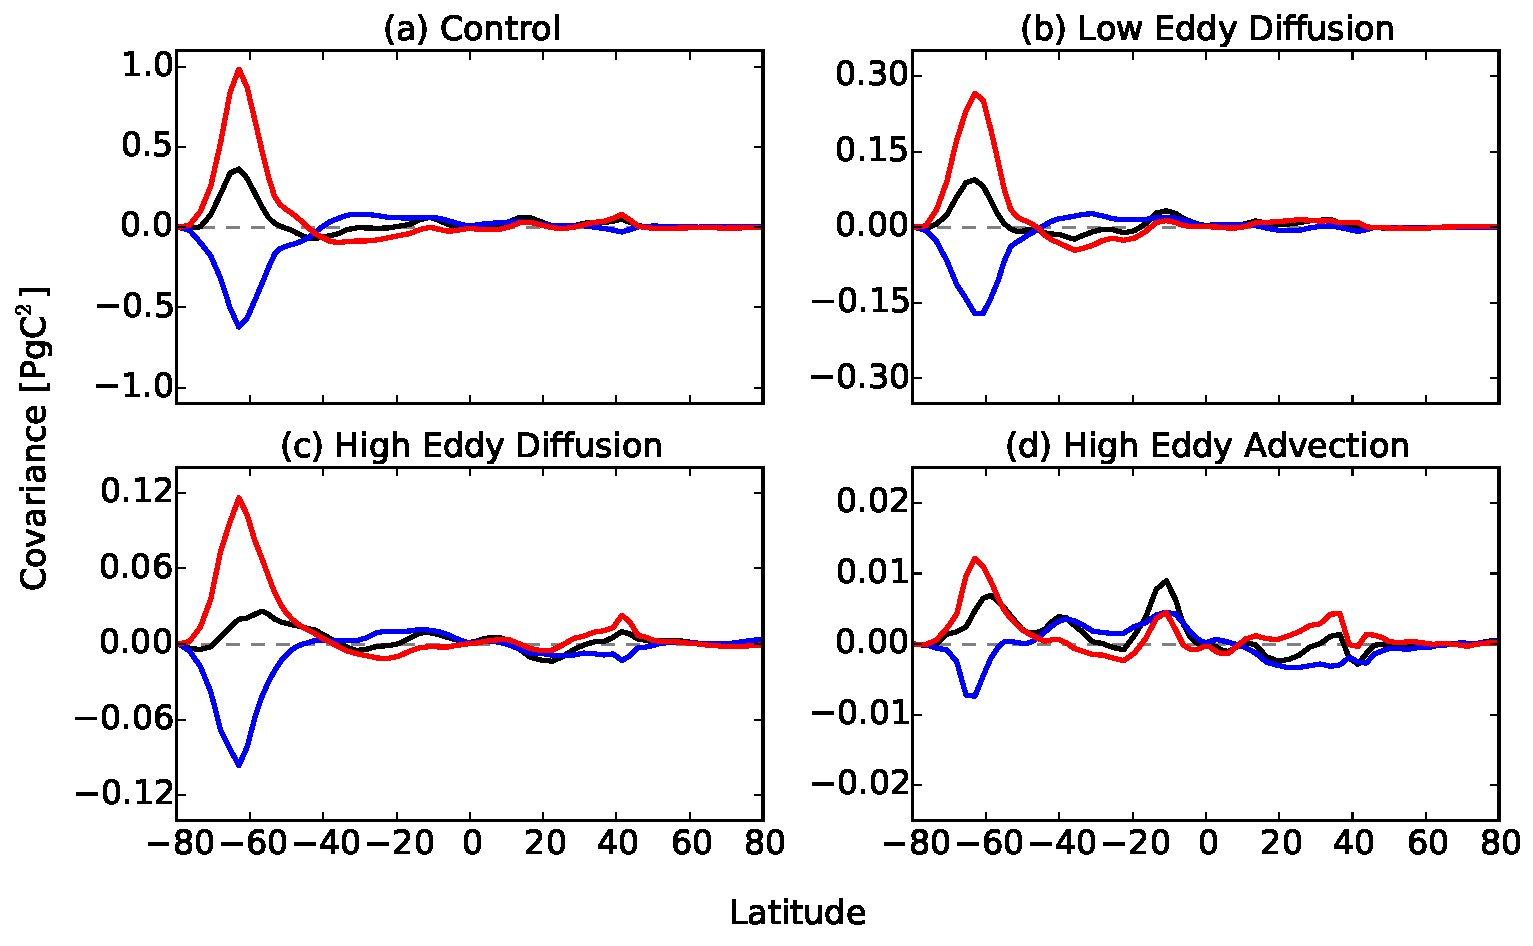
\includegraphics[width=33pc]{figure12.pdf}
\caption{Covariance between globally integrated DIC content and DIC (black),
preformed DIC (blue) and remineralized DIC (red) for each simulation as a
function of latitude. Note different y-axis scales.}
\label{fig:covariance}
\end{figure}

The opposite pattern holds for the covariance between global DIC
and preformed DIC: a negative covariance in the Southern Ocean, followed
by an increase in covariance in the southern mid-latitudes and a decrease below
zero north of the equator. Because of the lack of deep convection in the
\textit{high mixing simulations}, the Southern Ocean covariance is significantly smaller
than the other simulations (note different y-axis scales in
Figure~\ref{fig:covariance}), but the qualitative relationship remains the same.
The consistency in the general shape of these relationships suggests that the
same mechanisms are controlling the regional variability in all simulations.



%%%%%%%%%%%%%%%%%%%%%%%%%%%%%%%%%%%%%%%%%%%%%%%%%%%%%%%%%%%%%%%%%%%%%%%%%%%%%%%%
% CONCLUSIONS
%%%%%%%%%%%%%%%%%%%%%%%%%%%%%%%%%%%%%%%%%%%%%%%%%%%%%%%%%%%%%%%%%%%%%%%%%%%%%%%%

\section{Conclusions}
\label{section:conclusions}
Using a coupled climate model, we have quantified the global
and regional natural variability in oceanic heat and carbon content. We have
found that in this model, the highly convective Southern Ocean drives strong
global variability in heat and carbon content. Additionally, these two
quantities are strongly anti-correlated.  Using simulations with different
parameter settings for mesoscale mixing, we show that these results are robust
across simulations with different WS convective variability, but the
anti-correlation relationship is strongest with the two simulations which oscillate
between convecting and non-convecting states.

As illustrated in Figure~\ref{fig:schematic}, the global anti-correlation
between heat and carbon content is due to differences in the sign and magnitude
of the regional variability. The arrows in the schematic indicate the magnitude
of variability and the sign during a convective period. As indicated, the global
heat and carbon content are anti-correlated.

In the Southern Ocean, heat and
carbon content are both depleted during convection, but the southern
mid-latitude and tropical regions each have heat content variability that
balance the Southern Ocean variability. The resulting global heat content
variability therefore has the same sign and magnitude as the variability in the
southern mid-latitudes and tropics.
Carbon content variability on the other hand exhibits a cancelation between the
southern mid-latitudes and tropics. Therefore, the resulting variability in
global carbon content closely follows the variability in the Southern Ocean.


\begin{figure}
\noindent
\centering
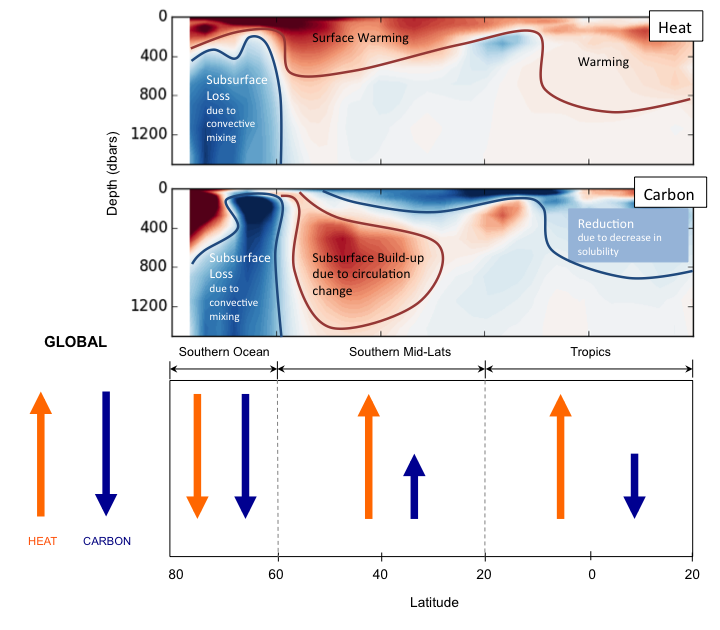
\includegraphics[width=1\linewidth]{schematic.png}
\caption{Schematic summarizing regional variability in oceanic heat and carbon
during a convective year. Arrows designate the sense of global and regional
inventory change during a convective year, positive indicating an increase in
oceanic content.}
\label{fig:schematic}
\end{figure}

The sub-surface variability structure is also depicted in Figure~\ref{fig:schematic}
and highlights the differences between heat and carbon.
During convection, both quantities decrease in the subsurface Southern Ocean.
Additionally, both heat and carbon show increases in the southern mid-latitudes,
but the temperature increases are contained in the surface, while DIC increases
at depth. This increase in subsurface DIC is likely a result of decreased
ventilation. Finally, the southern mid-latitudes and tropics show an increase in
surface temperature and a decrease in surface DIC. The variability in DIC here
is due to solubility decreases as a result of the temperature increase.

Comparing the magnitude of the modeled natural variability to the size of recent
observed trends can provide information on how detectible anthropogenic trends
are \citep{Thomas2015}. For the control simulations, the magnitude of global
carbon variability is about $\pm$ 3 PgC. This accounts for only approximately
3\% of the estimated anthropogenic uptake of carbon over the past few decades
\citep{Khatiwala2012,Sabine2004,Waugh2006}. The variability in global heat
content on the other hand is about $\pm$ 3 $\times 10^{22}$ J. This is a much
larger percentage (20\%) of the estimated uptake of anthropogenic heat in recent
decades \citep{Levitus2009}. These results suggest that changes in carbon
content due to anthropogenic activity are unlikely to be obscured by
long-timescale variability, but changes in heat content could be obscured. This
large natural variability in global heat content could explain why there is less
CMIP5 model agreement in oceanic heat uptake than there is for carbon uptake
\citep{Frolicher2009}.

If we assume these results hold for the real ocean, we would expect that during
the current non-convective period we would experience a subsurface warming in the Southern
Ocean and a slowdown of the intermediate water ventilation. Both these processes
have been documented in observational studies \citep{Purkey2012,Waugh2013b}, but
it is important to note that these changes could also be due to anthropogenic influences
such as greenhouse gas warming and ozone depletion in addition to variability in
WS convection.
The frequency of modeled WS convection is a hard to compare to real-life WS
convection because of the lack of an observational record in the Southern Ocean.
Additionally, \citet{DeLavergne2014a}
have shown that models that have frequent convection in preindustrial control
simulations have a significant reduction in convection under global warming
scenarios. This suggests that we may not observe another strong WS convective event,
and makes it extremely difficult to determine what frequency of WS convection is
`correct'.

The results of this study suggest that the atmosphere could exhibit significant
changes in temperature and CO$_2$ concentration in response to Southern Ocean
convective variability. A previous study by \citet{Cabre} using our
control version of the ESM2Mc model shows an increase in SH and global atmospheric
temperatures. This is because the additional flux of heat into the ocean is more
than balanced (and indeed is driven) by a decrease in clouds and ice, resulting
in an additional 0.15 PW of additional shortwave heating of the Southern Hemisphere
when convection is at its peak. An interesting extension of this
study would be to examine whether relatively small preindustrial changes in
atmospheric carbon dioxide could be associated with changes in SH temperatures,
as well as a more comprehensive examination of this process in Earth System
Models with variable atmospheric carbon dioxide.

A caveat with this study is that only a single model has been used. More
analysis should be conducted with additional model simulations to examine if
this relationship and the relative magnitudes of variability between heat and
carbon are consistent. Similar analysis with additional models could help to
understand the
intermodel spread of oceanic carbon content, and the larger intermodel spread
in  oceanic heat content \citep{Frolicher2014}, and also provide a better context
in which to analyze recent observational trends. Additionally, the model used in
this analysis has a relatively coarse resolution and parameterizations for
mesoscale eddies. \citet{Dufour2017} assessed the impact that model resolution has on
WS convection and concluded that horizontal model resolution has
an important impact on vertical stratification and the subsurface heat reservoir build-up.
However, the impact of resolution is not straightforward - a 1/4 degree ocean
behaved more like our high eddy diffusion model with relatively constant convection
while a 1/10 degree ocean model showed more stratification and behaved more
like our control model.
\citet{GRIFFIES2015} have additionally examined the impact eddies have on Southern
Ocean heat uptake and transport in eddy-permitting models
and have concluded that uncertain model
parameterizations tend to lead to model drift and less accurate lateral and
vertical heat distribution. These impacts need to be kept in mind when discussing
model simulations with parameterized eddies.



%\bibliography{/RESEARCH/library}
%%% Local Variables:
%%% mode: latex
%%% TeX-master: "thesis"
%%% End:
